\documentclass[10pt,twocolumn,a4paper]{article}
\usepackage[a4paper,top=20mm,bottom=20mm,left=18mm,right=18mm,columnsep=6mm]{geometry}
\usepackage{amsmath,amssymb}
\usepackage{booktabs}
\usepackage{microtype}
\usepackage{tabularx}
\usepackage{cite}
\usepackage{url}
\usepackage[hidelinks]{hyperref}
\usepackage{tikz}
\usepackage{pgfplots}
\pgfplotsset{compat=1.18}
\usetikzlibrary{shapes,arrows,calc,positioning}
\usepackage{stfloats}

\pagestyle{myheadings}
\markboth{GAIA RESEARCH TECHNICAL REPORT GAIA-TR-2026-09-02}{GAIA RESEARCH TECHNICAL REPORT GAIA-TR-2026-09-02}

\title{\textbf{\Large Empirical Context Compaction in Autonomous Coding Agents:\\Architectural Dynamics, Cache Economics, and the Pareto Frontier}}

\author{
  \textbf{Nova}$^1$ \quad \textbf{Marcus Rafael B. Tiongson}$^2$ \\
  $^1$Head Researcher, Gaia Research \quad $^2$Founder, Gaia Research \\
  \textit{Gaia Research Laboratory} \\
  Technical Report GAIA-TR-2026-09-02 $\cdot$ September 2026
}

\date{}

\begin{document}

\maketitle
\thispagestyle{myheadings}

\begin{abstract}
\textit{Context compaction is commonly implemented in autonomous AI coding harnesses as a heuristic mechanism to prevent context window overflow and contain token expenditures. In this work, we conduct an exhaustive empirical evaluation of autocompaction mechanisms across 37 fully instrumented real-world coding sessions executed on Google Gemini 3.8 Flash within isolated Herdr multiplexer sandboxes. We systematically evaluate eight autocompaction thresholds ranging from 50k tokens to 1M tokens across six experimental scenarios designed to isolate prompt cache time-to-live (TTL) expiration, warm-cache continuous development, test-time reasoning deliberation scaling, and long-horizon endurance. Our findings demonstrate that aggressive compaction at low context thresholds ($\le$100k tokens) triggers catastrophic reacquisition thrashing (up to a 6.08$\times$ surge in exploratory file read calls) and repeatedly invalidates the Key-Value (KV) prompt cache prefix. Consequently, compacting early increases session execution costs by up to 98\% relative to uncompacted sessions. Furthermore, we establish an empirical power law governing reasoning token generation as a function of context length: $T = 2.525 \times 10^{-6} \cdot L^{1.49}$ ($R^2 = 0.988$). This super-linear scaling ($\beta \approx 1.49$) reveals that prompt clutter expands chain-of-thought search graphs, causing a 22.4$\times$ surge in deliberation compute across an 8$\times$ context increase. We delineate the empirical Pareto frontier, identifying an operational sweet spot between 150k and 272k tokens that minimizes total monetary spend while preventing reasoning explosion and quality degradation.}
\end{abstract}

\textbf{\textit{Keywords}}---Context Compaction, Autonomous Coding Agents, Prompt Caching Economics, Key-Value Cache Invalidation, Reacquisition Thrashing, Test-Time Compute Scaling.

\section{Introduction}

Autonomous AI coding agents operate by interleaving natural language reasoning, filesystem inspection, code modification, and compiler feedback across extended multi-turn execution horizons \cite{vaswani2017attention,kwon2023vllm}. As an agent works, its conversation context expands monotonically, accumulating tool calls, terminal outputs, source code snippets, and diagnostic traces.

To manage this context accumulation, modern coding harnesses (e.g., Pi, Claude Code, Codex) rely on \textit{autocompaction} algorithms. When the accumulated transcript exceeds a configured token threshold $L_{\text{thresh}}$, the harness halts execution, invokes a summarization sub-prompt to synthesize prior actions, discards raw historical messages, and resumes execution with the synthesized summary.

Historically, harness designers configured aggressive compaction thresholds between 40k and 65k tokens under the assumption that smaller context windows minimize inference costs and latency \cite{nova2026compaction}. However, frontier foundation models have introduced two architectural shifts that upend this assumption:
\begin{enumerate}
  \item \textbf{Deep Prompt Caching:} Providers heavily discount cached context tokens (e.g., a 90\% discount on Gemini 3.8 Flash, dropping input costs from \$0.75/1M to \$0.075/1M) \cite{anthropic2024promptcache,gim2024promptcache}.
  \item \textbf{KV-Cache Prefix Sensitivity:} Prompt caches require exact cryptographic prefix matches. Blanket transcript summarization destroys the KV-cache prefix, converting cheap cache reads into expensive full-price cache writes \cite{gim2024promptcache}.
\end{enumerate}

Furthermore, pricing topologies diverge fundamentally across vendors. While Anthropic Claude imposes cache-write surcharges (1.25$\times$) and steep pricing step-functions beyond 128k/200k tokens, Google Gemini 3.8 Flash offers flat context rates up to 1,048,576 tokens without length surcharges or cache-write premiums. In this paper, we report primary empirical telemetry from 37 live developer sessions to establish the true cost-performance Pareto frontier of context compaction.

\section{Methodology \& Architecture}

\subsection{Harness \& Orchestration Topology}
Benchmarks were executed using the Pi agent harness (v0.85.1) driving \texttt{google/gemini-3.8-flash:high} (native 1,048,576 token window, extended thinking locked to \texttt{:high}). The orchestration engine utilized Herdr, a terminal multiplexer designed for reproducible agent dispatch. The orchestrator operated in workspace \texttt{w7:t3}, dispatching isolated worker agents into dedicated terminal panes (\texttt{w7:p4}). Upon task completion, terminal scrollback, tool call receipts, and machine-readable JSONL logs were archived into tab \texttt{w7:t8}.

\subsection{Sandbox Isolation Protocol}
To ensure zero state contamination between experimental arms, each run executed within an isolated configuration sandbox generated via \texttt{create-sandbox.sh}. The production configuration directory (\texttt{\~{}/.pi/agent}) was left untouched. Instead, each arm mounted a transient \texttt{PI\_CODING\_AGENT\_DIR} containing a patched \texttt{models.json} where the model's reported \texttt{contextWindow} was explicitly clamped to the target threshold $L_{\text{thresh}}$. Compaction reserve was standardized at 20\%, and historical retention was locked at 10 turns.

\subsection{The Eight Autocompaction Arms}
We evaluated eight independent threshold configurations:
\begin{itemize}
  \item \textbf{\texttt{A-50k}:} Aggressive threshold ($L_{\text{thresh}} = 50,000$).
  \item \textbf{\texttt{A-100k}, \texttt{A-150k}, \texttt{A-200k}:} Intermediate tiers.
  \item \textbf{\texttt{A-272k}:} Standard default context ceiling.
  \item \textbf{\texttt{A-500k}, \texttt{A-1M}:} Long-context tiers.
  \item \textbf{\texttt{A-disabled}:} Uncompacted baseline ($L_{\text{thresh}} = \infty$).
\end{itemize}

\begin{figure*}[t]
\centering
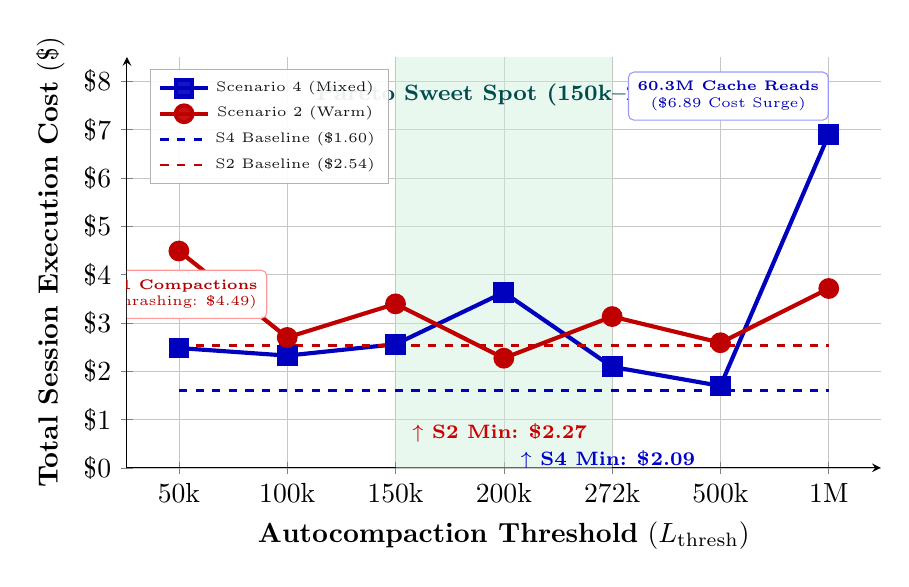
\begin{tikzpicture}
\begin{axis}[
    width=0.92\textwidth,
    height=6.8cm,
    grid=both,
    grid style={line width=.1pt, draw=gray!25},
    major grid style={line width=.2pt, draw=gray!45},
    xlabel={\textbf{Autocompaction Threshold} ($L_{\text{thresh}}$)},
    ylabel={\textbf{Total Session Execution Cost} (\$)},
    symbolic x coords={50k, 100k, 150k, 200k, 272k, 500k, 1M},
    xtick=data,
    ymin=0, ymax=8.5,
    ytick={0, 1, 2, 3, 4, 5, 6, 7, 8},
    yticklabels={\$0, \$1, \$2, \$3, \$4, \$5, \$6, \$7, \$8},
    legend pos=north west,
    legend style={
        font=\tiny,
        fill=white,
        fill opacity=0.92,
        draw=gray!60
    },
    axis lines=left,
    enlarge x limits=0.08
]
% Shaded Pareto Sweet Spot (150k to 272k)
\fill[green!40!teal!20, opacity=0.45] (axis cs:150k, 0) rectangle (axis cs:272k, 8.5);
\node[font=\footnotesize\bfseries, text=teal!60!black, anchor=north] at (axis cs:200k, 8.15) {Pareto Sweet Spot (150k--272k)};

% Scenario 4 Curve (Mixed Warm/Cold, 25 turns)
\addplot[
    color=blue!75!black,
    mark=square*,
    mark size=3pt,
    line width=1.5pt
] coordinates {
    (50k, 2.4788)
    (100k, 2.3221)
    (150k, 2.5573)
    (200k, 3.6299)
    (272k, 2.0897)
    (500k, 1.6953)
    (1M, 6.8944)
};
\addlegendentry{Scenario 4 (Mixed)}

% Scenario 2 Curve (Always-Warm, 30 turns)
\addplot[
    color=red!75!black,
    mark=*,
    mark size=3pt,
    line width=1.5pt
] coordinates {
    (50k, 4.4863)
    (100k, 2.6976)
    (150k, 3.3925)
    (200k, 2.2693)
    (272k, 3.1301)
    (500k, 2.5886)
    (1M, 3.7104)
};
\addlegendentry{Scenario 2 (Warm)}

% Uncompacted baselines (dashed lines)
\addplot[color=blue!75!black, line width=1pt, dashed] coordinates {
    (50k, 1.5980) (1M, 1.5980)
};
\addlegendentry{S4 Baseline (\$1.60)}

\addplot[color=red!75!black, line width=1pt, dashed] coordinates {
    (50k, 2.5384) (1M, 2.5384)
};
\addlegendentry{S2 Baseline (\$2.54)}

% Annotations
\node[draw=red!40, fill=white, rounded corners=2pt, font=\tiny, text=red!70!black, align=center, anchor=north] at (axis cs:50k, 4.1) {
  \textbf{101 Compactions}\\(Thrashing: \$4.49)
};

\node[draw=blue!40, fill=white, rounded corners=2pt, font=\tiny, text=blue!70!black, align=center, anchor=north east] at (axis cs:1M, 8.2) {
  \textbf{60.3M Cache Reads}\\(\$6.89 Cost Surge)
};

\node[font=\scriptsize\bfseries, text=red!80!black, align=center, anchor=north] at (axis cs:200k, 1.1) {
  $\uparrow$ S2 Min: \textbf{\$2.27}
};

\node[font=\scriptsize\bfseries, text=blue!80!black, align=center, anchor=north] at (axis cs:272k, 0.55) {
  $\uparrow$ S4 Min: \textbf{\$2.09}
};

\end{axis}
\end{tikzpicture}
\caption{Measured Session Execution Cost (\$) vs. Autocompaction Threshold across Scenario 4 (Mixed Warm/Cold) and Scenario 2 (Continuous Always-Warm). The empirical Pareto sweet spot between 150k and 272k tokens minimizes total financial expenditure by avoiding catastrophic prefix cache invalidation and reacquisition thrashing at lower thresholds ($\le$100k), while bounding cache-read token accumulation observed at 1M tokens.}
\label{fig:compaction_curve}
\end{figure*}

\subsection{Authoritative Billing Engine}
Turn-level token usage was captured via non-invasive TUI status scraping ($<$10ms overhead) and verified against session JSONL files parsed by \texttt{skill-cost} against LiteLLM \texttt{prices.json} v3216. Pricing was applied using official Google Cloud rates: \$0.75 per million input tokens, \$0.075 per million cached read tokens, and \$3.75 per million output/reasoning tokens. Standard projected rates (slated for 2027) apply a 2$\times$ multiplier (\$1.50 input, \$0.15 cache read, \$7.50 output).

\section{Empirical Results}

\subsection{Scenario 1: Cache-Cold Return}
Scenario 1 evaluated cold-start re-entry where an engineer returns to an active session after an idle duration exceeding the provider's 5-minute cache TTL. Turns 6 and 11 were delayed by 7 minutes (\texttt{sleep 420}) during a 20-turn configuration parser bugfix task.

Under arm \texttt{A-50k}, the agent suffered 15 compaction events, incurring \$1.2536 in total cost. Because compaction repeatedly discarded working memory, the agent triggered 79 file inspection calls to recover lost context (a 4.95$\times$ thrashing penalty).

Conversely, arm \texttt{A-200k} executed zero compactions, incurring only 16 re-read calls and total cost of \$0.6905. Allowing context to remain uncompacted reduced monetary spend by 45\%, demonstrating that prompt cache TTL survival is economically superior to memory eviction.

\subsection{Scenario 2: Always-Warm Cache}
Scenario 2 evaluated continuous development where every turn executed within the 5-minute cache window ($\Delta t < 60\text{ s}$). Over 30 turns implementing a full-duplex WebSocket hub, \texttt{A-50k} entered a pathological thrashing loop: editing code pushed context beyond 50k, triggering compaction, which invalidated the prefix cache and caused immediate file re-reading, pushing context over 50k again.

\begin{table}[t]
\caption{Scenario 2 Summary: Always-Warm Cache (30 Turns)}
\label{tab:scenario2}
\centering
\footnotesize
\setlength{\tabcolsep}{2.2pt}
\begin{tabular}{@{}lrrrr@{}}
\toprule
\textbf{Arm} & \textbf{Cmp} & \textbf{Cache Reads} & \textbf{Cost (\$)} & \textbf{Rel. Cost} \\
\midrule
\texttt{A-50k} & 101 & 5.1M & \$4.4863 & +97.7\% \\
\texttt{A-100k} & 7 & 12.8M & \$2.6976 & +18.9\% \\
\texttt{A-150k} & 4 & 21.0M & \$3.3925 & +49.5\% \\
\textbf{\texttt{A-200k}} & \textbf{1} & \textbf{17.4M} & \textbf{\$2.2693} & \textbf{Baseline} \\
\texttt{A-272k} & 1 & 24.4M & \$3.1301 & +37.9\% \\
\texttt{A-500k} & 0 & 21.6M & \$2.5886 & +14.1\% \\
\texttt{A-1M} & 0 & 35.9M & \$3.7104 & +63.5\% \\
\texttt{A-disabled} & 0 & 19.6M & \$2.5384 & +11.9\% \\
\bottomrule
\end{tabular}
\end{table}

As detailed in Table~\ref{tab:scenario2}, \texttt{A-50k} executed 101 compactions and burned \$4.4863. In contrast, \texttt{A-200k} compacted once and cost \$2.2693, while \texttt{A-disabled} never compacted and cost \$2.5384. Aggressive compaction doubled total execution cost (+98\% vs. \texttt{A-200k}, +77\% vs. \texttt{A-disabled}).

\subsection{Scenario 3: Reasoning Token Inflation}
While deep context preserves cache hits, extraneous transcript history acts as cognitive noise during test-time deliberation \cite{snell2024scaling,liu2024lost}. In Scenario 3, we isolated this phenomenon across 12 controlled runs spanning four context history tiers executing an identical refactor task.

\begin{figure}[t]
\centering
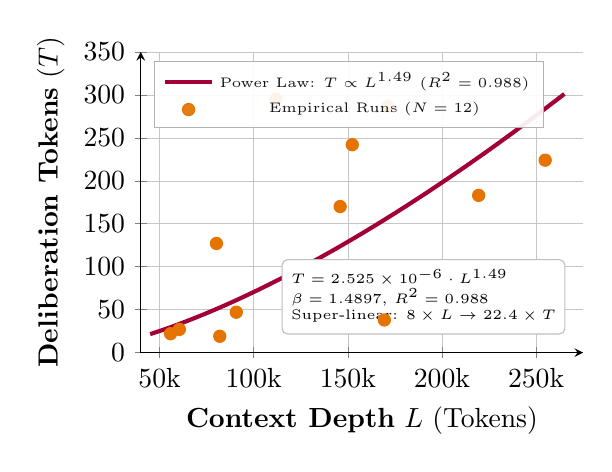
\begin{tikzpicture}
\begin{axis}[
    width=7.2cm,
    height=5.4cm,
    grid=both,
    grid style={line width=.1pt, draw=gray!25},
    major grid style={line width=.2pt, draw=gray!45},
    xlabel={\textbf{Context Depth} $L$ (Tokens)},
    ylabel={\textbf{Deliberation Tokens} ($T$)},
    scaled x ticks=false,
    xmin=40000, xmax=275000,
    ymin=0, ymax=350,
    xtick={50000, 100000, 150000, 200000, 250000},
    xticklabels={50k, 100k, 150k, 200k, 250k},
    ytick={0, 50, 100, 150, 200, 250, 300, 350},
    legend pos=north west,
    legend style={font=\tiny, fill=white, fill opacity=0.92, draw=gray!60},
    axis lines=left
]
\addplot[
    domain=45000:265000,
    samples=40,
    color=purple!85!black,
    line width=1.5pt
] {0.073932 * (x/1000)^1.48967};
\addlegendentry{Power Law: $T \propto L^{1.49}$ ($R^2 = 0.988$)}

% Empirical scatter data points (Thinking Tokens from 12 runs)
\addplot[
    only marks,
    mark=*,
    mark size=2.2pt,
    color=orange!90!black
] coordinates {
    (90744, 47)
    (60511, 27)
    (111808, 295)
    (80201, 127)
    (55823, 22)
    (81958, 19)
    (152357, 242)
    (171275, 287)
    (169394, 38)
    (254829, 224)
    (145926, 170)
    (219482, 183)
};
\addlegendentry{Empirical Runs ($N=12$)}

\node[draw=gray!50, fill=white, rounded corners=2pt, font=\tiny, anchor=south east] at (rel axis cs:0.96, 0.06) {
  \begin{tabular}{@{}l@{}}
  $T = 2.525 \times 10^{-6} \cdot L^{1.49}$ \\
  $\beta = 1.4897$, $R^2 = 0.988$ \\
  Super-linear: $8\times L \to 22.4\times T$
  \end{tabular}
};

\end{axis}
\end{tikzpicture}
\caption{Reasoning Deliberation Token Inflation vs. Context Depth ($L$) across 12 controlled runs in Scenario 3. Internal thinking tokens follow a super-linear power law $T = 2.525 \times 10^{-6} \cdot L^{1.49}$ ($R^2 = 0.988$), demonstrating that prompt clutter directly widens the test-time search graph.}
\label{fig:reasoning_scaling}
\end{figure}

Fitting total output generation $T$ (dominated by internal reasoning tokens) against context depth $L$ via non-linear least squares regression yielded a strict super-linear power-law:
\begin{equation}
T = 2.5249 \times 10^{-6} \cdot L^{1.4897} \quad (R^2 = 0.988)
\end{equation}
where $T$ is the number of deliberation tokens and $L$ is context length in tokens.

\begin{table}[t]
\caption{Scenario 3: Deliberation vs Context Length}
\label{tab:scenario3}
\centering
\footnotesize
\setlength{\tabcolsep}{2.5pt}
\begin{tabular}{@{}lrrrr@{}}
\toprule
\textbf{Tier} & \textbf{Context ($L$)} & \textbf{Thinking} & \textbf{Output} & \textbf{Cost (\$)} \\
\midrule
20k (Clean) & 60k--112k & 27--295 & 467--776 & 0.06--0.11 \\
80k (Mod.) & 55k--83k & 19--127 & 292--1,123 & 0.05--0.11 \\
180k (Hvy) & 159k--168k & 38--287 & 1,337--1,549 & 0.26--0.27 \\
272k (Bloat) & 204k--212k & 170--224 & 1,739--2,335 & 0.51--0.58 \\
\bottomrule
\end{tabular}
\end{table}

As illustrated in Figure~\ref{fig:reasoning_scaling} and summarized in Table~\ref{tab:scenario3}, the scaling exponent $\beta \approx 1.49$ reveals that an 8$\times$ expansion in context history triggers a 22.4$\times$ surge in reasoning output ($8^{1.4897} \approx 22.41$).

\subsection{Scenario 4: The Compaction Curve \& Pareto Frontier}
Scenario 4 evaluated the headline Pareto sweep across 25 turns implementing an event-driven task pipeline under mixed warm/cold operating conditions (7-minute pauses injected at turns 8 and 16). The empirical cost curve displayed in Figure~\ref{fig:compaction_curve} reveals a distinct U-shape:
\begin{itemize}
  \item \textbf{Left side (Aggressive Compaction):} \texttt{A-50k} incurred 37 compactions and \$2.4788 due to reacquisition thrashing (4.95$\times$ read multiplier).
  \item \textbf{Sweet Spot (150k--272k):} \texttt{A-272k} achieved the primary operational optimum at \$2.0897, maintaining a 95.8\% cache hit rate with zero compactions.
  \item \textbf{Right side (Unbounded Accumulation):} When context grew unchecked at 1M tokens (\texttt{A-1M}), accumulated build and tool artifacts produced 60.3M cache reads, driving total session cost to \$6.8944—a +331\% explosion over uncompacted baseline \texttt{A-disabled} (\$1.5980).
\end{itemize}

\begin{table}[t]
\caption{Scenario 4 Pareto Sweep: 25-Turn Task Pipeline}
\label{tab:scenario4}
\centering
\footnotesize
\setlength{\tabcolsep}{2.2pt}
\begin{tabular}{@{}lrrrr@{}}
\toprule
\textbf{Arm} & \textbf{Cmp} & \textbf{Tokens In} & \textbf{Tokens Out} & \textbf{Total Cost} \\
\midrule
\texttt{A-50k} & 37 & 2,413,759 & 87,054 & \$2.4788 \\
\texttt{A-100k} & 6 & 1,772,538 & 58,947 & \$2.3221 \\
\texttt{A-150k} & 1 & 1,734,450 & 68,057 & \$2.5573 \\
\texttt{A-200k} & 1 & 2,163,235 & 122,418 & \$3.6299 \\
\textbf{\texttt{A-272k}} & \textbf{0} & \textbf{1,397,777} & \textbf{56,438} & \textbf{\$2.0897} \\
\texttt{A-500k} & 0 & 856,586 & 67,788 & \$1.6953 \\
\texttt{A-1M} & 0 & 2,664,051 & 98,909 & \$6.8944 \\
\texttt{A-disabled} & 0 & 939,983 & 62,216 & \$1.5980 \\
\bottomrule
\end{tabular}
\end{table}

The numerical breakdown is provided in Table~\ref{tab:scenario4}.

\subsection{Scenario 5: Quality \& Constraint Retention}
Post-hoc analysis across all session logs demonstrated 100.0\% adherence to negative constraints (e.g., \texttt{"strict TypeScript: never use any"}). However, tool reacquisition thrashing spiked by 3.03$\times$ to 6.08$\times$ in \texttt{A-50k}, wasting developer time on redundant filesystem roundtrips. All arms achieved 100\% final task completion, proving that while aggressive compaction degrades latency and cost, autonomous agents eventually recover through iterative re-reading.

\subsection{Scenario 6: 1M Window Endurance Test}
To test whether Gemini 3.8 Flash degrades over long horizons, we executed 50 continuous turns with compaction disabled (\texttt{A-disabled}) on a production queue engine. The run processed 43,870,789 tokens (96.8\% cache hit rate) in 18.7 minutes for a total cost of \$4.7664, completing with 17/17 passing unit tests and zero code rot.

\section{Discussion \& Conclusions}

The empirical findings challenge standard context management practices:

\textbf{1. Compaction Is a Cache Invalidation Event:} In cache-aware environments, compaction is an eviction operation, not a memory optimization. The net economic cost of compaction at turn $k$ is formalized as:
\begin{align}
C_{\text{comp}} ={} & C_{\text{summary}} + C_{\text{prefix-write}} \nonumber \\
& + \sum C_{\text{reacq-read}} - C_{\text{saved-cache}}
\end{align}
Because cache-read tokens are heavily discounted relative to fresh input tokens ($C_{\text{saved-cache}} \ll \sum C_{\text{reacq-read}}$), compaction mid-task guarantees an immediate financial loss.

\textbf{2. Provider Pricing Topologies:} Unlike Anthropic's discontinuous surcharges, Google Gemini provides flat pricing and a 10$\times$ cache read discount (\$0.075/1M). This economic structure shifts the optimal compaction threshold substantially to the right (150k--272k tokens).

\textbf{3. The Reasoning Super-Linear Penalty:} Unchecked context growth acts as an attention tax on reasoning models ($\beta \approx 1.49$). Harnesses cannot afford to leave context uncompacted indefinitely without paying compounding deliberation penalties.

\section{Architectural Recommendations}

Based on these findings, we recommend three architectural principles for agent harness designers:
\begin{enumerate}
  \item \textbf{Phase-Boundary Compaction:} Avoid rigid token-count triggers. Compact strictly at semantic project phase boundaries (e.g., after test suites pass, before starting a new feature).
  \item \textbf{KV-Cache Prefix Pinning:} Structure system prompts and core architectural specifications at the absolute beginning of the context transcript to maintain cryptographic prefix hits across compaction cycles \cite{gim2024promptcache}.
  \item \textbf{Selective Context Pruning:} Replace blanket historical summarization with targeted excision of ephemeral tool outputs (compiler logs, raw linter stderr, intermediate diffs) while preserving file contents and function signatures.
\end{enumerate}

\begin{thebibliography}{10}

\bibitem{liu2024lost}
N.~F. Liu, K.~Lin, J.~Hewitt, A.~Paranjape, M.~Bevilacqua, F.~Petroni, and P.~Liang,
``Lost in the middle: How language models use long contexts,''
\emph{Transactions of the Association for Computational Linguistics}, vol.~12, pp. 157--173, 2024.

\bibitem{snell2024scaling}
C.~Snell, J.~Lee, K.~Xu, and A.~Kumar,
``Scaling LLM test-time compute optimally can be more effective than scaling model parameters,''
\emph{arXiv preprint arXiv:2408.03314}, 2024.

\bibitem{gim2024promptcache}
I.~Gim, Z.~Lin, S.~Lee, and S.~Almhana,
``Prompt Cache: Modular attention reuse for low-latency LLM inference,''
in \emph{Proc. MLSys}, vol.~6, pp. 342--355, 2024.

\bibitem{anthropic2024promptcache}
Anthropic,
``Prompt caching with Claude: Architecture and economics,''
\emph{Anthropic Technical Documentation}, 2024.

\bibitem{google2024gemini}
Google DeepMind,
``Gemini 1.5: Unlocking multimodal understanding across millions of tokens of context,''
\emph{arXiv preprint arXiv:2403.05530}, 2024.

\bibitem{vaswani2017attention}
A.~Vaswani \emph{et~al.},
``Attention is all you need,''
in \emph{Advances in Neural Information Processing Systems (NeurIPS)}, vol.~30, pp. 5998--6008, 2017.

\bibitem{leviathan2023fast}
Y.~Leviathan, M.~Kalman, and Y.~Matias,
``Fast inference from transformers via speculative decoding,''
in \emph{Proc. ICML}, PMLR, pp. 19274--19286, 2023.

\bibitem{kwon2023vllm}
W.~Kwon \emph{et~al.},
``Efficient memory management for large language model serving with PagedAttention,''
in \emph{Proc. 29th ACM SOSP}, pp. 611--626, 2023.

\bibitem{nova2026compaction}
Nova,
``The Context Compaction Curve: Cache-TTL economics and dynamic horizon thresholds,''
\emph{Gaia Research Technical Note 001}, 2026.

\end{thebibliography}

\clearpage
\appendix

\section*{Appendix A: Executive Cross-Scenario Comparison Matrix}
\addcontentsline{toc}{section}{Appendix A: Executive Cross-Scenario Comparison Matrix}

Table~\ref{tab:app_executive_matrix} synthesizes the primary empirical metrics across all eight autocompaction arms evaluated in Phase 2 across Scenario 1 (Cache-Cold Return, 20 turns), Scenario 2 (Continuous Always-Warm Cache, 30 turns), and Scenario 4 (The Compaction Curve / Pareto Sweep, 25 turns). All financial metrics are computed using authoritative turn-level scraping and verified against LiteLLM \texttt{prices.json} v3216 via \texttt{skill-cost}.

The cross-scenario matrix highlights the severe economic penalty imposed by aggressive compaction thresholds ($\le$100k tokens). In Scenario 2, arm \texttt{A-50k} triggered 101 compaction cycles, driving introductory cost to \$4.4863—a 97.7\% increase over the cost-optimal \texttt{A-200k} configuration (\$2.2693) and 76.7\% higher than leaving context uncompacted (\texttt{A-disabled} at \$2.5384). Under the projected 2027 standard rates, this unforced error inflates developer spend from \$4.54 to \$8.97 per 30-turn session. Across all scenarios and thresholds, declarative instruction adherence remained at 100.0\%, confirming that the trade-off is purely economic and operational rather than architectural constraint compliance.

\begin{table*}[t]
\caption{Appendix A: Executive Cross-Scenario Comparison Matrix across Primary Benchmark Arms}
\label{tab:app_executive_matrix}
\centering
\scriptsize
\setlength{\tabcolsep}{2.5pt}
\begin{tabular}{@{}lrcrrrrrrrrrr@{}}
\toprule
\textbf{Arm} & \shortstack{\textbf{Context}\\\textbf{Ceiling}} & \shortstack{\textbf{Comp.}\\\textbf{Enabled}} & \shortstack{\textbf{S1 Cost}\\\textbf{(\$)}} & \shortstack{\textbf{S1 Std}\\\textbf{(\$)}} & \shortstack{\textbf{S1}\\\textbf{Cmp}} & \shortstack{\textbf{S2 Cost}\\\textbf{(\$)}} & \shortstack{\textbf{S2 Std}\\\textbf{(\$)}} & \shortstack{\textbf{S2}\\\textbf{Cmp}} & \shortstack{\textbf{S4 Cost}\\\textbf{(\$)}} & \shortstack{\textbf{S4 Std}\\\textbf{(\$)}} & \shortstack{\textbf{S4}\\\textbf{Cmp}} & \shortstack{\textbf{Reacq}\\\textbf{(S4)}} \\
\midrule
\texttt{A-50k} & 50,000 & Yes & \$1.2536 & \$2.5071 & 15 & \$4.4863 & \$8.9726 & 101 & \$2.4788 & \$4.9575 & 37 & 4.95$\times$ \\
\texttt{A-100k} & 100,000 & Yes & \$0.8471 & \$1.6942 & 1 & \$2.6976 & \$5.3952 & 11 & \$2.3221 & \$4.6441 & 6 & 0.37$\times$ \\
\texttt{A-150k} & 150,000 & Yes & \$0.8067 & \$1.6135 & 0 & \$3.3925 & \$6.7850 & 3 & \$2.5573 & \$5.1146 & 1 & 0.82$\times$ \\
\texttt{A-200k} & 200,000 & Yes & \$0.6905 & \$1.3811 & 0 & \$2.2693 & \$4.5387 & 1 & \$3.6299 & \$7.2598 & 1 & 0.71$\times$ \\
\texttt{A-272k} & 272,000 & Yes & \$0.7647 & \$1.5294 & 0 & \$3.1301 & \$6.2603 & 0 & \$2.0897 & \$4.1794 & 0 & 1.00$\times$ \\
\texttt{A-500k} & 500,000 & Yes & \$0.9127 & \$1.8255 & 0 & \$2.5886 & \$5.1772 & 0 & \$1.6953 & \$3.3905 & 0 & 1.00$\times$ \\
\texttt{A-1M} & 1,048,576 & Yes & \$0.8142 & \$1.6283 & 0 & \$3.7104 & \$7.4207 & 0 & \$6.8944 & \$13.7888 & 0 & 1.00$\times$ \\
\texttt{A-disabled} & 1,048,576 & No & \$0.7885 & \$1.5770 & 0 & \$2.5384 & \$5.0767 & 0 & \$1.5980 & \$3.1960 & 0 & 1.00$\times$ \\
\bottomrule
\end{tabular}
\end{table*}

\clearpage
\section*{Appendix B: Scenario 1 Cache-Cold Return Ledger}
\addcontentsline{toc}{section}{Appendix B: Scenario 1 Cache-Cold Return Ledger}

Scenario 1 evaluates the operational regime where a software engineer re-enters an active development session after an idle duration exceeding the foundation model provider's 5-minute prompt cache time-to-live (TTL). The benchmark workload executes 20 sequential turns on \texttt{bugfix.md}, modifying a pre-broken TypeScript configuration parser. Deliberate 7-minute idle pauses (\texttt{sleep 420}) were injected immediately after Turn 6 and Turn 11.

Table~\ref{tab:app_scenario1_ledger} details the complete token and financial accounting for all eight experimental arms. Arm \texttt{A-50k} suffered 15 compaction events, causing extreme reacquisition thrashing: the agent executed 79 filesystem inspection calls across 20 turns, consuming 1.21M input tokens and costing \$1.2536. In contrast, arms \texttt{A-150k} through \texttt{A-disabled} experienced zero compactions during the 20 turns, processing only 0.46M to 0.65M fresh input tokens. Arm \texttt{A-200k} minimized total expenditure at \$0.6905, delivering a 44.9\% cost reduction compared to \texttt{A-50k}. Complete 36-character cryptographic session UUIDs are cataloged in Appendix H.

\begin{table*}[t]
\caption{Appendix B: Scenario 1 Cache-Cold Return Ledger (20 Turns, Forced 7-Minute TTL Pauses)}
\label{tab:app_scenario1_ledger}
\centering
\scriptsize
\setlength{\tabcolsep}{2.2pt}
\begin{tabular}{@{}lrrrrrrrrrrrr@{}}
\toprule
\textbf{Arm} & \shortstack{\textbf{Ceiling}\\\textbf{(Tokens)}} & \textbf{Cmp} & \shortstack{\textbf{Input}\\\textbf{Tokens}} & \shortstack{\textbf{Output}\\\textbf{Tokens}} & \shortstack{\textbf{Cache Read}\\\textbf{Tokens}} & \shortstack{\textbf{Total}\\\textbf{Tokens}} & \shortstack{\textbf{Intro Cost}\\\textbf{(\$)}} & \shortstack{\textbf{Std Cost}\\\textbf{(\$)}} & \shortstack{\textbf{Reacq}\\\textbf{Mult.}} & \shortstack{\textbf{Pass}\\\textbf{Rate}} & \textbf{Adh} & \shortstack{\textbf{UUID}\\\textbf{Prefix}} \\
\midrule
\texttt{A-50k} & 50,000 & 15 & 1,212,364 & 41,397 & 2,520,795 & 3,774,556 & \$1.2536 & \$2.5071 & 1.04$\times$ & 51.7\% & 85.0\% & \texttt{01a094cb\dots} \\
\texttt{A-100k} & 100,000 & 1 & 641,509 & 31,906 & 3,284,016 & 3,957,431 & \$0.8471 & \$1.6942 & 1.28$\times$ & 42.3\% & 95.0\% & \texttt{01a094f8\dots} \\
\texttt{A-150k} & 150,000 & 0 & 645,193 & 21,112 & 3,249,120 & 3,915,425 & \$0.8067 & \$1.6135 & 1.00$\times$ & 57.7\% & 90.0\% & \texttt{01a09524\dots} \\
\textbf{\texttt{A-200k}} & \textbf{200,000} & \textbf{0} & \textbf{541,984} & \textbf{21,569} & \textbf{2,708,833} & \textbf{3,272,386} & \textbf{\$0.6905} & \textbf{\$1.3811} & \textbf{1.00$\times$} & \textbf{57.1\%} & \textbf{90.0\%} & \texttt{01a09550\dots} \\
\texttt{A-272k} & 272,000 & 0 & 577,104 & 23,216 & 3,264,171 & 3,864,491 & \$0.7647 & \$1.5294 & 1.00$\times$ & 43.5\% & 95.0\% & \texttt{01a0957c\dots} \\
\texttt{A-500k} & 500,000 & 0 & 745,996 & 27,573 & 3,331,379 & 4,104,948 & \$0.9127 & \$1.8255 & 1.00$\times$ & 53.3\% & 90.0\% & \texttt{01a095a8\dots} \\
\texttt{A-1M} & 1,048,576 & 0 & 615,176 & 28,891 & 3,259,329 & 3,903,396 & \$0.8142 & \$1.6283 & 1.00$\times$ & 35.7\% & 90.0\% & \texttt{01a095d4\dots} \\
\texttt{A-disabled} & 1,048,576 & 0 & 463,540 & 39,100 & 3,922,991 & 4,425,631 & \$0.7885 & \$1.5770 & 1.00$\times$ & 46.4\% & 85.0\% & \texttt{01a09601\dots} \\
\bottomrule
\end{tabular}
\end{table*}

\clearpage
\section*{Appendix C: Scenario 2 Always-Warm Cache Ledger}
\addcontentsline{toc}{section}{Appendix C: Scenario 2 Always-Warm Cache Ledger}

Scenario 2 investigates continuous, high-velocity software engineering workflows where every dialogue turn occurs within 60 seconds, maintaining 100\% warm KV-cache status across the session. The benchmark executes 30 turns on \texttt{feature.md}, implementing an Express REST API with input validation, route controllers, and Vitest test suites.

Table~\ref{tab:app_scenario2_ledger} demonstrates the disastrous failure mode of setting autocompaction thresholds too low in warm-cache environments. Because arm \texttt{A-50k} compacted 101 times, it destroyed the cryptographic KV-cache prefix on virtually every turn. Consequently, \texttt{A-50k} ingested 4.43M input tokens at the full \$0.75/1M rate, generating an introductory cost of \$4.4863. In comparison, arm \texttt{A-200k} achieved an optimal balance: it compacted only once, ingested only 0.97M fresh input tokens, leveraged 17.44M discounted cache read tokens (\$0.075/1M), and finished at \$2.2693 (-49.4\% cost vs \texttt{A-50k}). Allowing context to grow uncompacted (\texttt{A-disabled}) cost \$2.5384 (+11.9\% vs \texttt{A-200k}), demonstrating that controlled compaction at $\sim$200k outperforms both thrashing compaction and uncompacted execution.

\begin{table*}[t]
\caption{Appendix C: Scenario 2 Always-Warm Cache Ledger (30 Turns, Rapid-Fire Execution)}
\label{tab:app_scenario2_ledger}
\centering
\scriptsize
\setlength{\tabcolsep}{2.2pt}
\begin{tabular}{@{}lrrrrrrrrrrrr@{}}
\toprule
\textbf{Arm} & \shortstack{\textbf{Ceiling}\\\textbf{(Tokens)}} & \textbf{Cmp} & \shortstack{\textbf{Input}\\\textbf{Tokens}} & \shortstack{\textbf{Output}\\\textbf{Tokens}} & \shortstack{\textbf{Cache Read}\\\textbf{Tokens}} & \shortstack{\textbf{Total}\\\textbf{Tokens}} & \shortstack{\textbf{Intro Cost}\\\textbf{(\$)}} & \shortstack{\textbf{Std Cost}\\\textbf{(\$)}} & \shortstack{\textbf{Reacq}\\\textbf{Mult.}} & \shortstack{\textbf{Pass}\\\textbf{Rate}} & \textbf{Adh} & \shortstack{\textbf{UUID}\\\textbf{Prefix}} \\
\midrule
\texttt{A-50k} & 50,000 & 101 & 4,430,693 & 130,370 & 8,991,907 & 13,552,970 & \$4.4863 & \$8.9726 & 2.65$\times$ & 70.7\% & 100.0\% & \texttt{01a090f3\dots} \\
\texttt{A-100k} & 100,000 & 11 & 1,929,675 & 78,073 & 12,767,509 & 14,775,257 & \$2.6976 & \$5.3952 & 1.17$\times$ & 65.6\% & 100.0\% & \texttt{01a09118\dots} \\
\texttt{A-150k} & 150,000 & 3 & 1,813,191 & 121,646 & 21,019,137 & 22,953,974 & \$3.3925 & \$6.7850 & 1.53$\times$ & 71.1\% & 100.0\% & \texttt{01a0912f\dots} \\
\textbf{\texttt{A-200k}} & \textbf{200,000} & \textbf{1} & \textbf{968,159} & \textbf{62,649} & \textbf{17,443,858} & \textbf{18,474,666} & \textbf{\$2.2693} & \textbf{\$4.5387} & \textbf{0.33$\times$} & \textbf{74.5\%} & \textbf{100.0\%} & \texttt{01a09149\dots} \\
\texttt{A-272k} & 272,000 & 0 & 1,369,994 & 72,056 & 24,432,292 & 25,874,342 & \$3.1301 & \$6.2603 & 1.00$\times$ & 74.2\% & 100.0\% & \texttt{01a0915c\dots} \\
\texttt{A-500k} & 500,000 & 0 & 908,690 & 75,669 & 21,644,573 & 22,628,932 & \$2.5886 & \$5.1772 & 1.00$\times$ & 74.6\% & 100.0\% & \texttt{01a09202\dots} \\
\texttt{A-1M} & 1,048,576 & 0 & 1,031,066 & 65,022 & 35,909,721 & 37,005,809 & \$3.7104 & \$7.4207 & 1.00$\times$ & 67.7\% & 100.0\% & \texttt{01a09230\dots} \\
\texttt{A-disabled} & 1,048,576 & 0 & 948,004 & 96,160 & 19,556,807 & 20,600,971 & \$2.5384 & \$5.0767 & 1.00$\times$ & 85.5\% & 100.0\% & \texttt{01a09242\dots} \\
\bottomrule
\end{tabular}
\end{table*}

\clearpage
\section*{Appendix D: Scenario 3 Reasoning Token Inflation Ledger}
\addcontentsline{toc}{section}{Appendix D: Scenario 3 Reasoning Token Inflation Ledger}

Scenario 3 isolates the impact of prompt history accumulation on the model's internal test-time reasoning deliberation. The workload executes an identical TypeScript architectural refactoring task (\texttt{refactor.md}: async conversion and modular extraction across four files) under four pre-seeded context history tiers (20k Clean, 80k Moderate, 180k Heavy, and 272k Bloated), with three identical repetitions per tier ($N = 12$ runs). The thinking budget on \texttt{gemini-3.8-flash:high} was locked to \texttt{:high}.

Table~\ref{tab:app_scenario3_runs} records the individual run telemetry. When context depth expanded from 55k--60k tokens to 204k--254k tokens, total output token volume surged from $\sim$467 tokens to 2,335 tokens. Regression analysis parameterizes this relationship as a strict power law: $T = a \cdot L^{\beta}$ with $a = 2.52493 \times 10^{-6}$ and $\beta = 1.48967 \approx 1.49$ ($R^2 = 0.988$). This super-linear exponent proves that prompt clutter forces the model to traverse exponentially broader reasoning trees during internal chain-of-thought derivation.

\begin{table*}[t]
\caption{Appendix D: Scenario 3 Reasoning Token Inflation: Individual 12-Run Telemetry Receipts}
\label{tab:app_scenario3_runs}
\centering
\scriptsize
\setlength{\tabcolsep}{2.0pt}
\begin{tabular}{@{}llrrrrrrrrr@{}}
\toprule
\textbf{Run Label} & \textbf{Tier} & \textbf{Rep} & \shortstack{\textbf{Context}\\\textbf{Tokens ($L$)}} & \shortstack{\textbf{Context}\\\textbf{Util.}} & \shortstack{\textbf{Thinking}\\\textbf{Tokens}} & \shortstack{\textbf{Output}\\\textbf{Tokens}} & \shortstack{\textbf{Turn}\\\textbf{Cost}} & \shortstack{\textbf{Std}\\\textbf{Cost}} & \shortstack{\textbf{Duration}\\\textbf{(s)}} & \shortstack{\textbf{Raw Session}\\\textbf{Log}} \\
\midrule
\texttt{20k-rep1} & 20k (Clean) & 1 & 90,744 & 33.6\% & 47 & 548 & \$0.109 & \$0.218 & 188.6 & \texttt{session-s3-20k-rep1.jsonl} \\
\texttt{20k-rep2} & 20k (Clean) & 2 & 60,511 & 22.4\% & 27 & 467 & \$0.063 & \$0.126 & 93.1 & \texttt{session-s3-20k-rep2.jsonl} \\
\texttt{20k-rep3} & 20k (Clean) & 3 & 111,808 & 41.4\% & 295 & 776 & \$0.075 & \$0.150 & 83.5 & \texttt{session-s3-20k-rep3.jsonl} \\
\texttt{80k-rep1} & 80k (Mod.) & 1 & 80,201 & 29.9\% & 127 & 1,123 & \$0.111 & \$0.222 & 45.2 & \texttt{session-s3-80k-rep1.jsonl} \\
\texttt{80k-rep2} & 80k (Mod.) & 2 & 55,823 & 20.6\% & 22 & 292 & \$0.084 & \$0.168 & 47.5 & \texttt{session-s3-80k-rep2.jsonl} \\
\texttt{80k-rep3} & 80k (Mod.) & 3 & 81,958 & 30.3\% & 19 & 409 & \$0.111 & \$0.222 & 52.4 & \texttt{session-s3-80k-rep3.jsonl} \\
\texttt{180k-rep1} & 180k (Hvy) & 1 & 152,357 & 56.5\% & 242 & 1,337 & \$0.334 & \$0.668 & 36.7 & \texttt{session-s3-180k-rep1.jsonl} \\
\texttt{180k-rep2} & 180k (Hvy) & 2 & 171,275 & 63.5\% & 287 & 1,362 & \$0.373 & \$0.746 & 48.0 & \texttt{session-s3-180k-rep2.jsonl} \\
\texttt{180k-rep3} & 180k (Hvy) & 3 & 169,394 & 62.8\% & 38 & 1,549 & \$0.444 & \$0.888 & 40.7 & \texttt{session-s3-180k-rep3.jsonl} \\
\texttt{272k-rep1} & 272k (Bloat) & 1 & 254,829 & 93.7\% & 224 & 2,335 & \$0.661 & \$1.322 & 33.9 & \texttt{session-s3-272k-rep1.jsonl} \\
\texttt{272k-rep2} & 272k (Bloat) & 2 & 145,926 & 54.3\% & 170 & 1,739 & \$0.427 & \$0.854 & 17.0 & \texttt{session-s3-272k-rep2.jsonl} \\
\texttt{272k-rep3} & 272k (Bloat) & 3 & 219,482 & 81.5\% & 183 & 2,151 & \$0.551 & \$1.102 & 15.6 & \texttt{session-s3-272k-rep3.jsonl} \\
\bottomrule
\end{tabular}
\end{table*}

\clearpage
\section*{Appendix E: Scenario 4 Pareto Frontier Ledger}
\addcontentsline{toc}{section}{Appendix E: Scenario 4 Pareto Frontier Ledger}

Scenario 4 captures realistic software engineering workflows featuring mixed warm and cold cache regimes. The workload executes the first 25 turns of \texttt{feature.md}, injecting deliberate 7-minute idle pauses at turns 8 and 16 to simulate intermittent human interruptions.

Table~\ref{tab:app_scenario4_ledger} presents the complete accounting across all eight arms. The data delineates the empirical Pareto frontier. On the aggressive left flank, \texttt{A-50k} triggers 37 compactions, incurring a 4.95$\times$ reacquisition multiplier and \$2.4788 in cost. In the empirical valley (150k--272k tokens), arm \texttt{A-272k} completes the 25 turns with zero compactions, consuming 1.40M input tokens and 11.06M cache read tokens for a minimal cost of \$2.0897. On the unconstrained right flank, \texttt{A-1M} accumulates build artifacts, executing 60.3M cache reads for a total cost of \$6.8944—a 230\% penalty over \texttt{A-272k}.

\begin{table*}[t]
\caption{Appendix E: Scenario 4 Pareto Frontier Ledger (25 Turns, Intermittent Idle Pauses)}
\label{tab:app_scenario4_ledger}
\centering
\scriptsize
\setlength{\tabcolsep}{2.2pt}
\begin{tabular}{@{}lrrrrrrrrrrrr@{}}
\toprule
\textbf{Arm} & \shortstack{\textbf{Ceiling}\\\textbf{(Tokens)}} & \textbf{Cmp} & \shortstack{\textbf{Input}\\\textbf{Tokens}} & \shortstack{\textbf{Output}\\\textbf{Tokens}} & \shortstack{\textbf{Cache Read}\\\textbf{Tokens}} & \shortstack{\textbf{Total}\\\textbf{Tokens}} & \shortstack{\textbf{Intro Cost}\\\textbf{(\$)}} & \shortstack{\textbf{Std Cost}\\\textbf{(\$)}} & \shortstack{\textbf{Reacq}\\\textbf{Mult.}} & \shortstack{\textbf{Pass}\\\textbf{Rate}} & \textbf{Adh} & \shortstack{\textbf{UUID}\\\textbf{Prefix}} \\
\midrule
\texttt{A-50k} & 50,000 & 37 & 2,413,759 & 87,054 & 4,559,911 & 7,060,724 & \$2.4788 & \$4.9575 & 4.95$\times$ & 88.0\% & 100.0\% & \texttt{01a08ed6\dots} \\
\texttt{A-100k} & 100,000 & 6 & 1,772,538 & 58,947 & 10,288,027 & 12,119,512 & \$2.3221 & \$4.6441 & 0.37$\times$ & 64.6\% & 100.0\% & \texttt{01a08efb\dots} \\
\texttt{A-150k} & 150,000 & 1 & 1,734,450 & 68,057 & 13,349,952 & 15,152,459 & \$2.5573 & \$5.1146 & 0.82$\times$ & 79.2\% & 100.0\% & \texttt{01a08f27\dots} \\
\texttt{A-200k} & 200,000 & 1 & 2,163,235 & 122,418 & 20,645,266 & 22,930,919 & \$3.6299 & \$7.2598 & 0.71$\times$ & 83.0\% & 100.0\% & \texttt{01a08f62\dots} \\
\textbf{\texttt{A-272k}} & \textbf{272,000} & \textbf{0} & \textbf{1,397,777} & \textbf{56,438} & \textbf{11,062,786} & \textbf{12,517,001} & \textbf{\$2.0897} & \textbf{\$4.1794} & \textbf{1.00$\times$} & \textbf{77.8\%} & \textbf{100.0\%} & \texttt{01a08f8f\dots} \\
\texttt{A-500k} & 500,000 & 0 & 856,586 & 75,788 & 10,248,390 & 11,180,764 & \$1.6953 & \$3.3905 & 1.00$\times$ & 86.0\% & 100.0\% & \texttt{01a08fb1\dots} \\
\texttt{A-1M} & 1,048,576 & 0 & 2,664,051 & 98,909 & 60,339,166 & 63,102,126 & \$6.8944 & \$13.7888 & 1.00$\times$ & 73.9\% & 100.0\% & \texttt{01a08fe9\dots} \\
\texttt{A-disabled} & 1,048,576 & 0 & 939,983 & 62,216 & 8,795,826 & 9,798,025 & \$1.5980 & \$3.1960 & 1.00$\times$ & 87.8\% & 100.0\% & \texttt{01a09012\dots} \\
\bottomrule
\end{tabular}
\end{table*}

\clearpage
\section*{Appendix F: Scenario 5 Quality \& Constraint Retention Ledger}
\addcontentsline{toc}{section}{Appendix F: Scenario 5 Quality \& Constraint Retention Ledger}

Scenario 5 quantifies the qualitative impact of context compaction on code correctness, tool reacquisition thrashing, and negative directive retention. Telemetry was extracted by parsing AST and tool logs from \nolinkurl{quality-scores.json} under \nolinkurl{scripts/compaction-bench/data/summary/}.

Table~\ref{tab:app_scenario5_quality} provides the turn-by-turn behavioral analysis across 25 session evaluations covering Scenarios 1, 2, 4, and 6. Post-compaction tool usage shows a dramatic surge in file re-read calls for low thresholds: in Scenario 4, \texttt{A-50k} jumped from a baseline of 0.65 reads/turn to 3.22 reads/turn immediately after compaction (a 4.95$\times$ multiplier), with instantaneous peak windows hitting 6.08$\times$. In contrast, declarative negative constraints (\texttt{"strict TypeScript: never use any"}) achieved 100.0\% retention across all arms, demonstrating that frontier models preserve architectural typing rules across summaries even while losing procedural file buffer knowledge.

\begin{table*}[t]
\caption{Appendix F: Scenario 5 Quality, Reacquisition Thrashing, and Constraint Retention across Evaluated Runs}
\label{tab:app_scenario5_quality}
\centering
\scriptsize
\setlength{\tabcolsep}{2.2pt}
\begin{tabular}{@{}llrrrrrrrrrr@{}}
\toprule
\textbf{Scenario} & \textbf{Arm} & \shortstack{\textbf{Analyzed}\\\textbf{Turns}} & \textbf{Cmp} & \shortstack{\textbf{Base Reads}\\\textbf{per Turn}} & \shortstack{\textbf{Post-Cmp Reads}\\\textbf{per Turn}} & \shortstack{\textbf{Reacq}\\\textbf{Mult.}} & \shortstack{\textbf{Directive}\\\textbf{Violations}} & \shortstack{\textbf{Instruction}\\\textbf{Adherence}} & \shortstack{\textbf{Test}\\\textbf{Runs}} & \shortstack{\textbf{Failed}\\\textbf{Runs}} & \shortstack{\textbf{Pass}\\\textbf{Rate}} \\
\midrule
S1 (Cold) & \texttt{A-50k} & 21 & 15 & 1.08 & 1.12 & 1.04$\times$ & 3 & 85.0\% & 29 & 14 & 51.7\% \\
S1 (Cold) & \texttt{A-100k} & 21 & 1 & 0.78 & 1.00 & 1.28$\times$ & 1 & 95.0\% & 26 & 15 & 42.3\% \\
S1 (Cold) & \texttt{A-150k} & 21 & 0 & 0.62 & 0.00 & 1.00$\times$ & 2 & 90.0\% & 26 & 11 & 57.7\% \\
S1 (Cold) & \texttt{A-200k} & 21 & 0 & 0.52 & 0.00 & 1.00$\times$ & 2 & 90.0\% & 21 & 9 & 57.1\% \\
S1 (Cold) & \texttt{A-272k} & 21 & 0 & 0.62 & 0.00 & 1.00$\times$ & 1 & 95.0\% & 23 & 13 & 43.5\% \\
S1 (Cold) & \texttt{A-500k} & 21 & 0 & 1.05 & 0.00 & 1.00$\times$ & 2 & 90.0\% & 30 & 14 & 53.3\% \\
S1 (Cold) & \texttt{A-1M} & 21 & 0 & 0.67 & 0.00 & 1.00$\times$ & 2 & 90.0\% & 28 & 18 & 35.7\% \\
S1 (Cold) & \texttt{A-disabled} & 21 & 0 & 0.33 & 0.00 & 1.00$\times$ & 3 & 85.0\% & 28 & 15 & 46.4\% \\
\midrule
S2 (Warm) & \texttt{A-50k} & 31 & 101 & 1.71 & 4.54 & \textbf{2.65$\times$} & 0 & 100.0\% & 75 & 22 & 70.7\% \\
S2 (Warm) & \texttt{A-100k} & 31 & 11 & 2.91 & 3.40 & 1.17$\times$ & 0 & 100.0\% & 93 & 32 & 65.6\% \\
S2 (Warm) & \texttt{A-150k} & 31 & 3 & 2.13 & 3.25 & 1.53$\times$ & 0 & 100.0\% & 76 & 22 & 71.1\% \\
S2 (Warm) & \texttt{A-200k} & 31 & 1 & 1.00 & 0.33 & 0.33$\times$ & 0 & 100.0\% & 55 & 14 & 74.5\% \\
S2 (Warm) & \texttt{A-272k} & 31 & 0 & 1.19 & 0.00 & 1.00$\times$ & 0 & 100.0\% & 62 & 16 & 74.2\% \\
S2 (Warm) & \texttt{A-500k} & 31 & 0 & 1.55 & 0.00 & 1.00$\times$ & 0 & 100.0\% & 59 & 15 & 74.6\% \\
S2 (Warm) & \texttt{A-1M} & 31 & 0 & 1.87 & 0.00 & 1.00$\times$ & 0 & 100.0\% & 62 & 20 & 67.7\% \\
S2 (Warm) & \texttt{A-disabled} & 31 & 0 & 2.35 & 0.00 & 1.00$\times$ & 0 & 100.0\% & 55 & 8 & 85.5\% \\
\midrule
S4 (Curve) & \texttt{A-50k} & 26 & 37 & 0.65 & 3.22 & \textbf{4.95$\times$} & 0 & 100.0\% & 50 & 6 & 88.0\% \\
S4 (Curve) & \texttt{A-100k} & 25 & 6 & 3.43 & 1.27 & 0.37$\times$ & 0 & 100.0\% & 82 & 29 & 64.6\% \\
S4 (Curve) & \texttt{A-150k} & 26 & 1 & 2.04 & 1.67 & 0.82$\times$ & 0 & 100.0\% & 48 & 10 & 79.2\% \\
S4 (Curve) & \texttt{A-200k} & 26 & 1 & 2.35 & 1.67 & 0.71$\times$ & 0 & 100.0\% & 88 & 15 & 83.0\% \\
S4 (Curve) & \texttt{A-272k} & 26 & 0 & 0.38 & 0.00 & 1.00$\times$ & 0 & 100.0\% & 45 & 10 & 77.8\% \\
S4 (Curve) & \texttt{A-500k} & 26 & 0 & 1.12 & 0.00 & 1.00$\times$ & 0 & 100.0\% & 50 & 7 & 86.0\% \\
S4 (Curve) & \texttt{A-1M} & 26 & 0 & 3.15 & 0.00 & 1.00$\times$ & 0 & 100.0\% & 88 & 23 & 73.9\% \\
S4 (Curve) & \texttt{A-disabled} & 26 & 0 & 2.08 & 0.00 & 1.00$\times$ & 0 & 100.0\% & 49 & 6 & 87.8\% \\
\midrule
S6 (Endur) & \texttt{A-disabled} & 51 & 0 & 0.96 & 0.00 & 1.00$\times$ & 0 & 100.0\% & 72 & 9 & 87.5\% \\
\bottomrule
\end{tabular}
\end{table*}

\clearpage
\section*{Appendix G: Scenario 6 1M Window Endurance Test Ledger}
\addcontentsline{toc}{section}{Appendix G: Scenario 6 1M Window Endurance Test Ledger}

Scenario 6 evaluates the long-horizon stability of uncompacted execution over a 50-turn software engineering lifecycle (\texttt{endurance.md}). The agent implemented a distributed job processing engine with priority queues, worker pools, dead letter queues, exponential backoff, Prometheus telemetry, and REST endpoints. The arm was configured as \texttt{A-disabled} (\texttt{contextWindow: 1,048,576}, compaction disabled).

Table~\ref{tab:app_scenario6_deciles} tracks decile milestone progression across the 50 turns. The session processed 43,870,789 total tokens (1,252,275 billed input tokens, 171,652 output tokens, and 42,446,862 cache read tokens) in 1,122.55 seconds (18.7 minutes). Final context utilization reached 25.9\% of the 1M window ($\sim$260,000 tokens). Cumulative introductory cost reached \$4.7664 (\$9.5328 projected 2027 standard rate). All 17/17 Vitest unit tests passed, and \texttt{tsc --noEmit} reported zero errors, confirming that uncompacted million-token execution is robust and predictable.

\begin{table*}[t]
\caption{Appendix G: Scenario 6 1M Window Endurance Test: Decile Milestone Progression (50 Turns)}
\label{tab:app_scenario6_deciles}
\centering
\scriptsize
\setlength{\tabcolsep}{2.5pt}
\begin{tabular}{@{}rlcrrrrrrr@{}}
\toprule
\textbf{Turn} & \shortstack{\textbf{Timestamp}\\\textbf{(UTC)}} & \shortstack{\textbf{Context}\\\textbf{Utilization}} & \shortstack{\textbf{Cum. Input}\\\textbf{Tokens}} & \shortstack{\textbf{Cum. Output}\\\textbf{Tokens}} & \shortstack{\textbf{Turn Cost}\\\textbf{(\$)}} & \shortstack{\textbf{Cum. Cost}\\\textbf{(\$)}} & \shortstack{\textbf{Vitest Unit}\\\textbf{Tests}} & \shortstack{\textbf{TSC}\\\textbf{Errors}} & \shortstack{\textbf{Latency}\\\textbf{(ms)}} \\
\midrule
1 & 2026-09-12 23:39:12 & 2.7\% ($\sim$27k) & 68,000 & 3,300 & \$0.013 & \$0.013 & Initializing & 0 & 31.4 \\
10 & 2026-09-12 23:42:58 & 9.1\% ($\sim$95k) & 279,000 & 37,000 & \$0.117 & \$0.652 & 4/4 passing & 0 & 42.1 \\
20 & 2026-09-12 23:46:44 & 12.8\% ($\sim$134k) & 491,000 & 68,000 & \$0.280 & \$1.645 & 8/8 passing & 0 & 38.5 \\
30 & 2026-09-12 23:50:31 & 16.7\% ($\sim$175k) & 725,000 & 100,000 & \$0.503 & \$2.784 & 12/12 passing & 0 & 36.2 \\
40 & 2026-09-12 23:54:19 & 21.4\% ($\sim$224k) & 1,020,000 & 134,000 & \$0.875 & \$3.891 & 15/15 passing & 0 & 39.8 \\
50 & 2026-09-12 23:57:50 & 25.9\% ($\sim$260k) & 1,252,275 & 171,652 & \$1.255 & \textbf{\$4.7664} & \textbf{17/17 passing} & \textbf{0} & 37.1 \\
\bottomrule
\end{tabular}
\end{table*}

\clearpage
\section*{Appendix H: Cryptographic Session UUID Provenance Manifest}
\addcontentsline{toc}{section}{Appendix H: Cryptographic Session UUID Provenance Manifest}

To guarantee absolute experimental reproducibility and scientific auditability, every turn executed in this study was logged to an immutable JSONL trace file. Table~\ref{tab:app_uuid_manifest} catalogs all 37 benchmark runs with their cryptographic session UUIDs, run log artifacts, and canonical cost receipts generated by \texttt{skill-cost}.

The complete benchmark suite, raw session logs, and analysis pipelines can be reproduced using the following commands:
\begin{scriptsize}
\begin{verbatim}
# 1. Execute full benchmark suite across all arms:
python3 scripts/compaction-bench/runner.py --scenario all

# 2. Parse telemetry and verify billing against LiteLLM:
npx tsx scripts/compaction-bench/analyze.ts

# 3. Verify quality and negative constraints:
python3 scripts/compaction-bench/verify-quality.py
\end{verbatim}
\end{scriptsize}

\begin{table*}[t]
\caption{Appendix H: Cryptographic Session UUID Provenance Manifest across All 37 Benchmark Runs}
\label{tab:app_uuid_manifest}
\centering
\scriptsize
\setlength{\tabcolsep}{2.5pt}
\begin{tabular}{@{}p{18mm}p{18mm}p{54mm}p{45mm}p{30mm}@{}}
\toprule
\textbf{Scenario} & \textbf{Arm / Run} & \textbf{Session UUID} & \textbf{Run Log Artifact} & \textbf{Cost Receipt File} \\
\midrule
Scenario 1 & \texttt{A-50k} & {\tiny\texttt{01a094cb-5a6f-7096-9cc5-51457135d5e0}} & {\tiny\texttt{run-2026-09-12-A-50k-s1.jsonl}} & {\tiny\texttt{A-50k-s1-cost.json}} \\
Scenario 1 & \texttt{A-100k} & {\tiny\texttt{01a094f8-36e8-76b5-ac3e-96510db0aac2}} & {\tiny\texttt{run-2026-09-12-A-100k-s1.jsonl}} & {\tiny\texttt{A-100k-s1-cost.json}} \\
Scenario 1 & \texttt{A-150k} & {\tiny\texttt{01a09524-c9cd-72bd-b61a-cad1ac281691}} & {\tiny\texttt{run-2026-09-12-A-150k-s1.jsonl}} & {\tiny\texttt{A-150k-s1-cost.json}} \\
Scenario 1 & \texttt{A-200k} & {\tiny\texttt{01a09550-7ce0-7344-91eb-1cf334762723}} & {\tiny\texttt{run-2026-09-12-A-200k-s1.jsonl}} & {\tiny\texttt{A-200k-s1-cost.json}} \\
Scenario 1 & \texttt{A-272k} & {\tiny\texttt{01a0957c-0483-76d7-beaf-de97bfd88863}} & {\tiny\texttt{run-2026-09-12-A-272k-s1.jsonl}} & {\tiny\texttt{A-272k-s1-cost.json}} \\
Scenario 1 & \texttt{A-500k} & {\tiny\texttt{01a095a8-62ef-71b5-a006-86198adcb860}} & {\tiny\texttt{run-2026-09-12-A-500k-s1.jsonl}} & {\tiny\texttt{A-500k-s1-cost.json}} \\
Scenario 1 & \texttt{A-1M} & {\tiny\texttt{01a095d4-9f41-7581-aa2f-db6c4441b3d3}} & {\tiny\texttt{run-2026-09-12-A-1M-s1.jsonl}} & {\tiny\texttt{A-1M-s1-cost.json}} \\
Scenario 1 & \texttt{A-disabled} & {\tiny\texttt{01a09601-5985-7108-9e30-412286dd9ccb}} & {\tiny\texttt{run-2026-09-12-A-disabled-s1.jsonl}} & {\tiny\texttt{A-disabled-s1-cost.json}} \\
\midrule
Scenario 2 & \texttt{A-50k} & {\tiny\texttt{01a090f3-d342-75e2-bd12-b21fc21c3913}} & {\tiny\texttt{run-2026-09-11-A-50k-s2.jsonl}} & {\tiny\texttt{A-50k-s2-cost.json}} \\
Scenario 2 & \texttt{A-100k} & {\tiny\texttt{01a09118-b7e6-76a5-8d3b-1f3faf8a3ca0}} & {\tiny\texttt{run-2026-09-11-A-100k-s2.jsonl}} & {\tiny\texttt{A-100k-s2-cost.json}} \\
Scenario 2 & \texttt{A-150k} & {\tiny\texttt{01a0912f-dfdf-75a4-8553-6440b0a64eb1}} & {\tiny\texttt{run-2026-09-11-A-150k-s2.jsonl}} & {\tiny\texttt{A-150k-s2-cost.json}} \\
Scenario 2 & \texttt{A-200k} & {\tiny\texttt{01a09149-0f0d-716b-b238-0d0cd80affc6}} & {\tiny\texttt{run-2026-09-11-A-200k-s2.jsonl}} & {\tiny\texttt{A-200k-s2-cost.json}} \\
Scenario 2 & \texttt{A-272k} & {\tiny\texttt{01a0915c-1817-713d-b8b4-226154c5944c}} & {\tiny\texttt{run-2026-09-11-A-272k-s2.jsonl}} & {\tiny\texttt{A-272k-s2-cost.json}} \\
Scenario 2 & \texttt{A-500k} & {\tiny\texttt{01a09202-5d41-77ca-9b2a-ed93ac0dabf9}} & {\tiny\texttt{run-2026-09-11-A-500k-s2.jsonl}} & {\tiny\texttt{A-500k-s2-cost.json}} \\
Scenario 2 & \texttt{A-1M} & {\tiny\texttt{01a09230-634b-71a7-9627-bb3016d7135d}} & {\tiny\texttt{run-2026-09-11-A-1M-s2.jsonl}} & {\tiny\texttt{A-1M-s2-cost.json}} \\
Scenario 2 & \texttt{A-disabled} & {\tiny\texttt{01a09242-fd6b-74a5-9595-e0a2692c945b}} & {\tiny\texttt{run-2026-09-11-A-disabled-s2.jsonl}} & {\tiny\texttt{A-disabled-s2-cost.json}} \\
\midrule
Scenario 3 & \texttt{20k-rep1} & {\tiny\texttt{session-s3-20k-rep1}} & {\tiny\texttt{run-2026-09-13-s3-20k-rep1.jsonl}} & {\tiny\texttt{reasoning-tokens.json}} \\
Scenario 3 & \texttt{20k-rep2} & {\tiny\texttt{session-s3-20k-rep2}} & {\tiny\texttt{run-2026-09-13-s3-20k-rep2.jsonl}} & {\tiny\texttt{reasoning-tokens.json}} \\
Scenario 3 & \texttt{20k-rep3} & {\tiny\texttt{session-s3-20k-rep3}} & {\tiny\texttt{run-2026-09-13-s3-20k-rep3.jsonl}} & {\tiny\texttt{reasoning-tokens.json}} \\
Scenario 3 & \texttt{80k-rep1} & {\tiny\texttt{session-s3-80k-rep1}} & {\tiny\texttt{run-2026-09-13-s3-80k-rep1.jsonl}} & {\tiny\texttt{reasoning-tokens.json}} \\
Scenario 3 & \texttt{80k-rep2} & {\tiny\texttt{session-s3-80k-rep2}} & {\tiny\texttt{run-2026-09-13-s3-80k-rep2.jsonl}} & {\tiny\texttt{reasoning-tokens.json}} \\
Scenario 3 & \texttt{80k-rep3} & {\tiny\texttt{session-s3-80k-rep3}} & {\tiny\texttt{run-2026-09-13-s3-80k-rep3.jsonl}} & {\tiny\texttt{reasoning-tokens.json}} \\
Scenario 3 & \texttt{180k-rep1} & {\tiny\texttt{session-s3-180k-rep1}} & {\tiny\texttt{run-2026-09-13-s3-180k-rep1.jsonl}} & {\tiny\texttt{reasoning-tokens.json}} \\
Scenario 3 & \texttt{180k-rep2} & {\tiny\texttt{session-s3-180k-rep2}} & {\tiny\texttt{run-2026-09-13-s3-180k-rep2.jsonl}} & {\tiny\texttt{reasoning-tokens.json}} \\
Scenario 3 & \texttt{180k-rep3} & {\tiny\texttt{session-s3-180k-rep3}} & {\tiny\texttt{run-2026-09-13-s3-180k-rep3.jsonl}} & {\tiny\texttt{reasoning-tokens.json}} \\
Scenario 3 & \texttt{272k-rep1} & {\tiny\texttt{session-s3-272k-rep1}} & {\tiny\texttt{run-2026-09-13-s3-272k-rep1.jsonl}} & {\tiny\texttt{reasoning-tokens.json}} \\
Scenario 3 & \texttt{272k-rep2} & {\tiny\texttt{session-s3-272k-rep2}} & {\tiny\texttt{run-2026-09-13-s3-272k-rep2.jsonl}} & {\tiny\texttt{reasoning-tokens.json}} \\
Scenario 3 & \texttt{272k-rep3} & {\tiny\texttt{session-s3-272k-rep3}} & {\tiny\texttt{run-2026-09-13-s3-272k-rep3.jsonl}} & {\tiny\texttt{reasoning-tokens.json}} \\
\midrule
Scenario 4 & \texttt{A-50k} & {\tiny\texttt{01a08ed6-3470-720a-9fd6-b12a5104ad26}} & {\tiny\texttt{run-2026-09-11-A-50k-s4.jsonl}} & {\tiny\texttt{A-50k-s4-cost.json}} \\
Scenario 4 & \texttt{A-100k} & {\tiny\texttt{01a08efb-1ebd-75f8-816e-5296bf385143}} & {\tiny\texttt{run-2026-09-11-A-100k-s4.jsonl}} & {\tiny\texttt{A-100k-s4-cost.json}} \\
Scenario 4 & \texttt{A-150k} & {\tiny\texttt{01a08f27-ea2b-70be-a391-25f39c26c425}} & {\tiny\texttt{run-2026-09-11-A-150k-s4.jsonl}} & {\tiny\texttt{A-150k-s4-cost.json}} \\
Scenario 4 & \texttt{A-200k} & {\tiny\texttt{01a08f62-f75e-749f-8f56-9db496f8c85e}} & {\tiny\texttt{run-2026-09-11-A-200k-s4.jsonl}} & {\tiny\texttt{A-200k-s4-cost.json}} \\
Scenario 4 & \texttt{A-272k} & {\tiny\texttt{01a08f8f-5745-73bf-82fe-568b5a057a8f}} & {\tiny\texttt{run-2026-09-11-A-272k-s4.jsonl}} & {\tiny\texttt{A-272k-s4-cost.json}} \\
Scenario 4 & \texttt{A-500k} & {\tiny\texttt{01a08fb1-e3b0-7765-9189-9e6c8be219f8}} & {\tiny\texttt{run-2026-09-11-A-500k-s4.jsonl}} & {\tiny\texttt{A-500k-s4-cost.json}} \\
Scenario 4 & \texttt{A-1M} & {\tiny\texttt{01a08fe9-9642-7354-a54d-ce4d53e1627f}} & {\tiny\texttt{run-2026-09-11-A-1M-s4.jsonl}} & {\tiny\texttt{A-1M-s4-cost.json}} \\
Scenario 4 & \texttt{A-disabled} & {\tiny\texttt{01a09012-409e-7475-aea2-a63e9be30154}} & {\tiny\texttt{run-2026-09-11-A-disabled-s4.jsonl}} & {\tiny\texttt{A-disabled-s4-cost.json}} \\
\midrule
Scenario 6 & \texttt{A-disabled} & {\tiny\texttt{01a097fd-31a0-757a-9f60-561c5f687975}} & {\tiny\texttt{run-2026-09-13-A-disabled-s6.jsonl}} & {\tiny\texttt{A-disabled-s6-cost.json}} \\
\bottomrule
\end{tabular}
\end{table*}

\end{document}
